\documentclass[10pt, letterpaper, twoside]{article}
\usepackage[utf8]{inputenc}
\usepackage{ geometry }
\geometry{margin=1.5cm}
\usepackage{ amssymb }
\usepackage{ bbm }
\usepackage{ braket }
\usepackage{ mathrsfs }
\usepackage{ geometry }
\usepackage{ amsmath }
\usepackage[alphabetic]{ amsrefs }
\usepackage{ hyperref }
\usepackage{ enumitem }
\usepackage{ graphicx }
\usepackage{ multicol }
\setlength{\columnsep}{0.8cm}
\usepackage{ blindtext }
\usepackage{ caption }
\usepackage{ bookmark }
\usepackage{ float }
\usepackage{pgf, tikz}

\newenvironment{Figure}
  {\par\medskip\noindent\minipage{\linewidth}}
  {\endminipage\par\medskip}

\newcommand{\s}{L-system}


\makeatletter
\renewcommand{\maketitle}{\bgroup\setlength{\parindent}{0pt}
\begin{flushleft}
  \textbf{\@title}

  \@author
\end{flushleft}\egroup
}
\makeatother

\title{\Large L-systems - IG3D assignment}

\author{\Large Hugo Thomas\\ \small Quantum Information, Sorbonne Université}

\begin{document}

\maketitle

\begin{multicols}{2}

\paragraph{Foreword:}In this short report, I will make a quick review of
L-systems, relying on the book The algorithmic beauty of plants \cite{TheAB},
without talking about the code implementation. Since I'm not an IMA master
student, i.e. I'm not familiar with computer graphics and the fact that the
project has to be done in a quite short time, I have just explored in depth the
first three chapters of the book, i.e. the first ...  pages. Moreover, the
theoretical tools have not changed since the release of the book, it fully
covers the state-of-the-art. I will simply explain part of its content. Finally,
it is not possible to sum up the whole state-of-the-art in a three-pages review,
that is why I have carefully chosen to explain only the parts that are the most
interesting to me.

\section*{L-Systems}
This section presents the simplest class of L-systems, those which are
deterministic and context-free, called D0L-systems. One could define L-systems
as a formal way of defining developmental processes, that suits well to organic
models, and especially plant-development models. More formally, an L-system $G$ is
defined as a tuple $\langle V, \omega, P \rangle$, where $V$ is the alphabet of
symbols, $\omega \in V^+$ is the axiom, and $P \subset V \times V^*$ is the set
of production rules, also called rewriting rules: it takes a character $c \in V$
and returns a string $s \in V^*$. The axiom is the starting character of the
L-system, that will fully determine the iteration process. Let $s_i$ be the
result of the $i^{th}$ iteration, we define $s_0 = \omega$. An iteration
consists of the transformation $s_i \rightarrow s_{i+1}$ defined by the
successive transformations of the characters of $s_i$ according to the
production set $P$. \\\noindent For the sake of simplicity, if $x$ and $y$ are
two string in $V^*$, then $xy$ is the concatenation of $x$ and $y$.
\paragraph*{Example:}
Let $G_1 = \langle V, \omega, P \rangle$, where $V = \{A,B\}; \omega = A; P =
\{A\rightarrow AB, B\rightarrow BA\}$. Then the iterations go as follows:

\begin{equation}
    \begin{aligned}
        s_0 &= \omega = A \\
        s_1 &= P(A) = AB \\
        s_2 &= P(A)P(B) \\
            &= ABBA \\
        s_3 &= P(A)P(B)P(B)P(A)\\
            &= ABBABAAB
    \end{aligned}
\end{equation}

It almost fully describes an \s, we now need to interpret the result of an
iteration.
\section*{Turtle}
Turtle graphics, firstly defined by the Logo programming language \cite{Logo} is
a descriptive way of defining computer drawings. We can hence consider an
interpretation of some characters (not necessarily all of them) of the alphabet.
This will make the turtle move on the screen, and hence draw. For example, $F$
moves forward a step $l$, $+$ turns clockwise the turtle of an angle $\delta$,
and $-$ turns counterclockwise the turtle of an angle $\delta$.
\paragraph{Example:} If we let $l=1, \delta = 90$, and consider the sentence
$FFF+FF+F+F-F-FF+FFF$, then the turtle graphics formalism yields the following,
starting in $(0,0)$:
\begin{Figure}
    \centering
    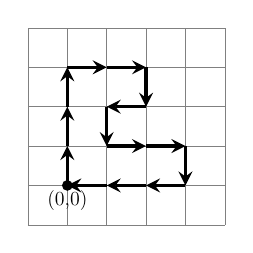
\begin{tikzpicture}[thick,scale=0.5, every node/.style={scale=0.5}]
        \draw [step=1.0,gray, very thin] (-1,-1) grid (4, 4);
        \draw [step=1.0,black, very thick, -stealth](0, 0) -- (0, 1);
        \draw [step=1.0,black, very thick, -stealth](0, 1) -- (0, 2);
        \draw [step=1.0,black, very thick, -stealth](0, 2) -- (0, 3);
        \draw [step=1.0,black, very thick, -stealth](0, 3) -- (1, 3);
        \draw [step=1.0,black, very thick, -stealth](1, 3) -- (2, 3);
        \draw [step=1.0,black, very thick, -stealth](2, 3) -- (2, 2);
        \draw [step=1.0,black, very thick, -stealth](2, 2) -- (1, 2);
        \draw [step=1.0,black, very thick, -stealth](1, 2) -- (1,1);
        \draw [step=1.0,black, very thick, -stealth](1, 1) -- (2,1);
        \draw [step=1.0,black, very thick, -stealth](2, 1) -- (3,1);
        \draw [step=1.0,black, very thick, -stealth](3, 1) -- (3, 0);
        \draw [step=1.0,black, very thick, -stealth](3, 0) -- (2, 0);
        \draw [step=1.0,black, very thick, -stealth](2, 0) -- (1, 0);
        \draw [step=1.0,black, very thick, -stealth](1, 0) -- (0,0);
        \filldraw[black] (0,0) circle (3pt) node[anchor=north]{\Large(0,0)};
    \end{tikzpicture}
    \captionof{figure}{Example of turtle drawing.}
\end{Figure}

By combining the L-System formalism and the turtle graphics, one can easily
generate fractal like patterns, thanks to the recursive structure of L-systems. ($n$ is
the number of iterations)

\begin{Figure}
    \centering
    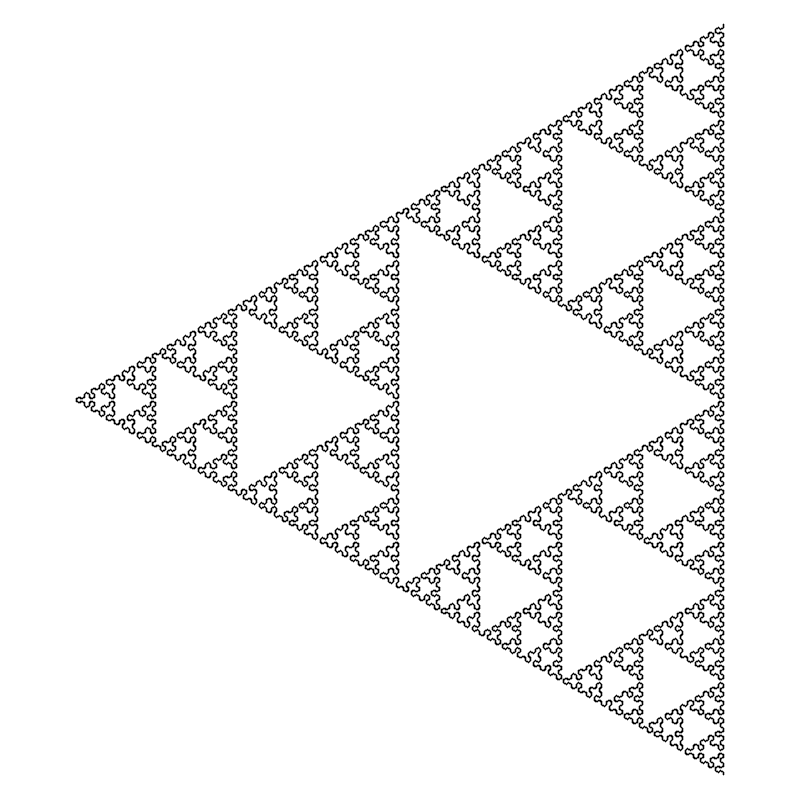
\includegraphics[width=0.7\linewidth, angle=-90]{img/triangle.png}
    \captionof{figure}{Fractal-like L-system model, $n=8$, def. \ref{app:tri}}
    \label{fig:triangle}
\end{Figure}

Fig. \ref{fig:triangle} shows a fractal-like model where each pattern repeats
itself, this comes from the recursive manner of defining an iteration.

\section*{More realistic L-systems}
This definition of L-systems yields interesting and fractal-like results, but we
need to add a branching possibility in order to obtain plant-like results. This
is achieved by considering a stack of turtle \textit{states} and its associated
operations: $\texttt{Push}$ and $\texttt{Pop}$. Those two operations are usually
represented by the characters $[$ and $]$ respectively. This enhancement yield
results shown in Fig. \ref{fig:fuzzy} and \ref{fig:aglae}.

\begin{Figure}
    \centering
    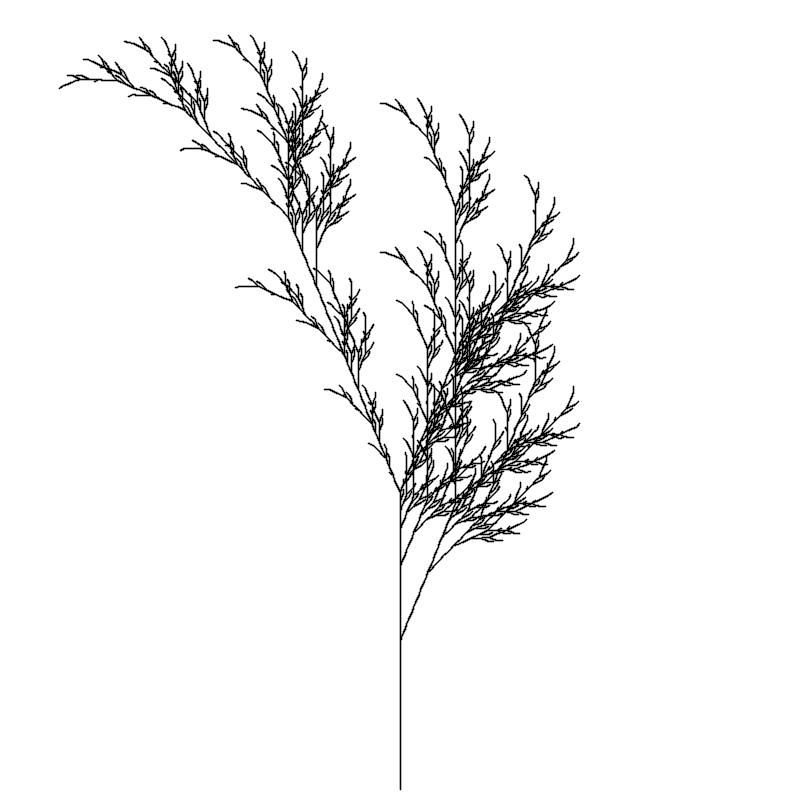
\includegraphics[scale=0.2]{img/fuzzy.png}
    \captionof{figure}{Fuzzy tree, $n=7$, def. \ref{app:fuzzy}}
    \label{fig:fuzzy}
\end{Figure}

The plant-like pattern appears directly, however, we will explore some
enhancement techniques in order to make those more realistic. The issue that one
faces with this kind of \textit{very simple} L-system, is that the plant
generated by a L-system is unique, and the artificial regularity is striking. To solve
this problem, it is possible to randomize the turtle parameters, the L-system
or both.

Randomizing only the turtle parameters has the effect of letting the underlying
structure of the results unchanged, while randomizing the L-system itself
probabilistically changes the structure, which has the effect of making the result
more realistic. Combining the two options is in the end the preferable solution.
Such a result is shown in Fig. \ref{fig:randomized}.

\begin{Figure}
    \centering
    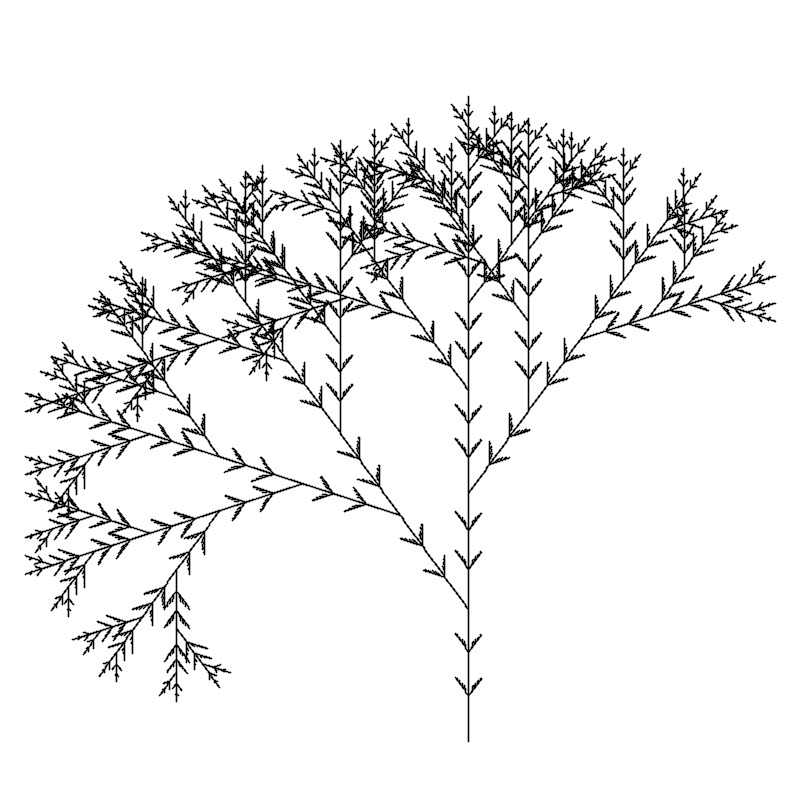
\includegraphics[scale=0.2]{img/aglae.png}
    \captionof{figure}{Aglae, $n=18$}
    \label{fig:aglae}
\end{Figure}

The list of species being described by L-systems grammar is vastly increasing.
Models have been made: cucumber growth \cite{cucumber}, sunflower \cite{TheAB}
(see Fig. \ref{fig:sunflower}), barley \cite{barley}, sorghum \cite{sorghum}.

\begin{Figure}
    \centering
    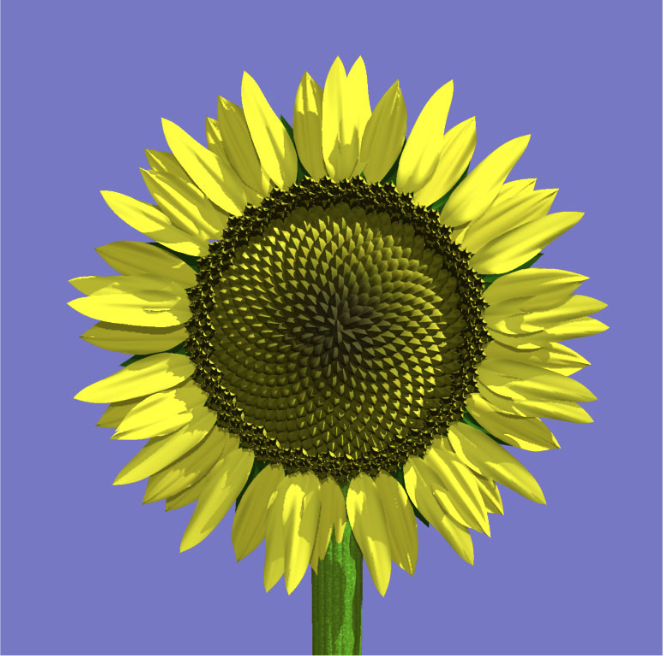
\includegraphics[scale=0.2]{img/sunflower.png}
    \captionof{figure}{ The famous sunflower of Prusinkiewicz and Lindenmayer,
        described by an L-system of only 8 lines of code.}
    \label{fig:sunflower}
\end{Figure}

\begin{Figure}
    \centering
    \begin{minipage}{.3\textwidth}
      \centering
      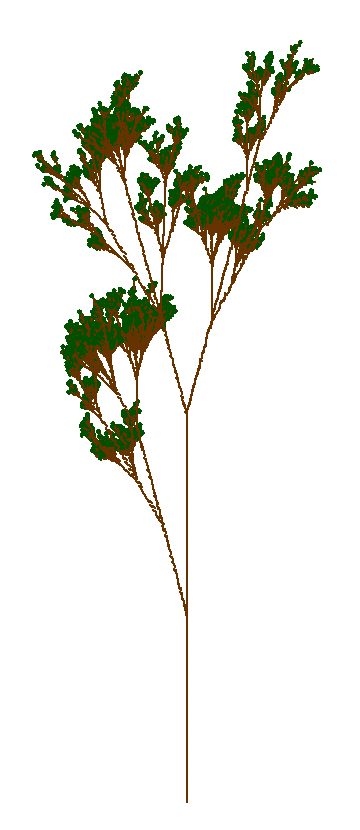
\includegraphics[width=1\linewidth]{img/r-tree-1.png}
    %   \label{fig:test1}
    \end{minipage}%
    \begin{minipage}{.3\textwidth}
      \centering
      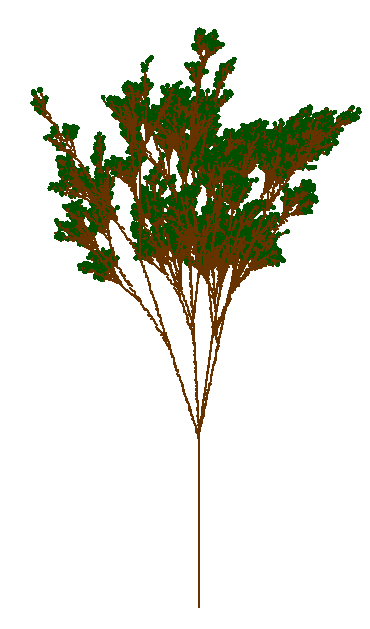
\includegraphics[width=1\linewidth]{img/r-tree-2.png}
    %   \captionof{figure}{Another figure}
    %   \label{fig:test2}
    \end{minipage}
    \begin{minipage}{.3\textwidth}
        \centering
        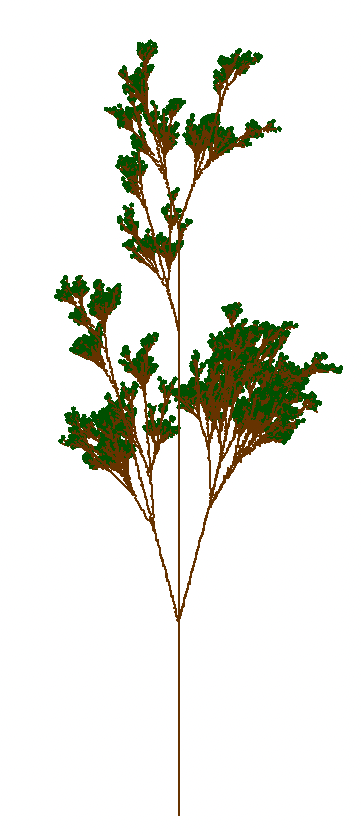
\includegraphics[width=1\linewidth]{img/r-tree-3.png}
        % \captionof{figure}{Another figure}
        % \label{fig:test3}
    \end{minipage}

    \captionof{figure}{Results generated by a stochastic L-system, $n=8$}
    \label{fig:randomized}
\end{Figure}

\section*{Developmental models of herbaceous plants}
In the case of self-similar structures, like trees illustrated in Fig.
\ref{fig:fuzzy} \ref{fig:aglae} \ref{fig:randomized}, the synthesis methods
based on rewriting rules, are fairly expressive and randomizing strategies fix
the problem of unnatural regularity. However, a more general approach is needed
to model the large variety of developmental patterns and structures found in
nature, especially, it is not possible to obtain Fig. \ref{fig:sunflower} only
with 0L-systems. When one observes nature, one sees that the flower development
is, although repetitive, highly controlled. For instance, in most of the cases
when a flower grows, the stem grows first, and in the end the flower appears.
Partial L-systems offer this possibility, especially for the case of
single-flower shoot.

\subsubsection*{Partial L-systems}
Partial L-systems can express the vegetative growth of a plant and, after a
certain time, the production of the flower. It's not in essence a new kind of
L-systems, in the sense that it is completely defined by a stochastic L-system,
but arises from the interpretation of these. Considering the example given in
\cite{TheAB} :
\begin{equation}
    \label{eq:partial}
    \begin{aligned}
        \omega & : a \\
        a \rightarrow &
        \begin{cases}
            I [L] a & \text{w.p. } \alpha\\
            I [L] A & \text{w.p. } \beta
        \end{cases} \\
        A \rightarrow & K
    \end{aligned}
\end{equation}
We of course have to have $\alpha + \beta = 1$, $\alpha, \beta \geq 0$. The
flower stays in its vegetative phase as long as the rule $a\rightarrow I[L]a$ is
applied, and once the rule $a\rightarrow I[L]A$ is selected, the shot stops and
the flower appears. It is hence possible to control the average height of the
flower, by controlling the ratio $\frac{\alpha}{\beta}$, that can be interpreted
as the average height of the result as shown in Fig. \ref{fig:partial}. Note
that the number of iterations is an upper-bound, since the rule $a\rightarrow
I[L]A$ is blocking.

\begin{Figure}
    \centering
    \begin{minipage}{.3\textwidth}
      \centering
      
\includegraphics[width=0.2\linewidth]{img/f-1.png}
    \end{minipage}%
    \begin{minipage}{.3\textwidth}
      \centering
      
\includegraphics[width=0.2\linewidth]{img/f-4.png}
    \end{minipage}%
    \begin{minipage}{.3\textwidth}
        \centering
        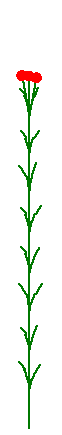
\includegraphics[width=0.2\linewidth]{img/f-3.png}
    \end{minipage}
    \captionof{figure}{Partial L-system results, $n=6$, def.(\ref{eq:partial})}
    \label{fig:partial}
\end{Figure}

\subsubsection*{Context-sensitive L-systems}
Unlike the 0L-systems in which production rules are applied regardless of the
context, context-sensitive L-systems, apply rules depending on the context of
the character evaluated, that is, its predecessors and successors. This effect is
useful in simulating interactions between plant parts. We thus introduce
production rules of the form $a_l < a > a_r \rightarrow \chi$, where the rule $a
\rightarrow \chi$ is applied if and only if $a$ is preceded by $a_l$ and
followed by $a_r$. This allows to \textit{move} characters (see example), and
then introduce a sort of timer in the process. Systems in which we consider only
one side for the context are denoted 1L-systems, and the one where we consider
the two neighbors of a character, as the following example, are called
2L-systems.

\paragraph{Example (from \cite{TheAB}, shortened):}
\begin{equation}
    \begin{aligned}
        \omega & : baaa \\
        b<a & \rightarrow b\\
        a<b> \emptyset & \rightarrow f\\
        b & \rightarrow a \\
    \end{aligned}
\end{equation}
The first generated sentences are given below:
\begin{equation}
        baaa \Rightarrow % \quad;\quad
        abaa \Rightarrow % \quad;\quad
        aaba \Rightarrow % \quad;\quad
        aaab \Rightarrow % \quad;\quad
        aaaf \quad
\end{equation}

\paragraph{Note:} The priority of the rule application not is given by their
order of definition, but by the range of their context the broadest context is
given priority.

After the $4^{th}$ iteration, the character $f$ appears at the end of the
sentence, meaning that if we associate $f$ to the flower and $a$ to the stem,
then the flower appears after four iterations at the top of the stem. It is
easy, starting from this example, to infer how one can use context-sensitive
L-systems to create flower-like models.

\section*{Open problems - Miscellaneous}

An interesting application of parametric context-sensitive L-systems has been
exposed by Hammel and Prusinkiewicz \cite{diff-eq}, is the use of those systems
to express numerical solutions to initial value problems for partial
differential equation.
\\

Every 0L-system $G$ defines an obvious set of derivations $E(G)$. Those
objects, the \textit{0L sequence languages} have been studied in
\cite{ROZENBERG1980195}.\\
\textbf{Open problem:} Given two arbitrary OL-systems $G_1$ and $G_2$, is it
possible to decide whether $E(G_1) = E(G_2)$?\\R. Book conjectured that the
answer to the above question is positive. \\

A locally contenative sequence is a sequence of words in which each word can be
constructed as the concatenation of previous words in the sequence.\\
\textbf{Open problem:} Is it decidable whether an arbitrary DOL-system is
locally contenative ?

The above problem constitutes today perhaps the most important open
problem concerning DOL systems.

\bibliographystyle{alpha}
\bibliography{bibliography}
\newpage
\appendix
\section{L-systems definitions}\label{app:ldef}
\subsection{Triangle}\label{app:tri}
Parameters:
\begin{equation}
    \begin{aligned}
        l & =10 \\
        \delta & = 60 \\
    \end{aligned}
\end{equation}
System:
\begin{equation}
    \begin{aligned}
        \omega & : A \\
        \\
        B & \rightarrow -A+B+A- \\
        A & \rightarrow +B-A-B+ \\
    \end{aligned}
\end{equation}

\subsection{Fuzzy tree}\label{app:fuzzy}
Parameters:
\begin{equation}
    \begin{aligned}
        l & =10 \\
        \delta & = 22 \\
    \end{aligned}
\end{equation}
System:
\begin{equation}
    \begin{aligned}
        \omega & : X \\
        \\
        F & \rightarrow FF \\
        X & \rightarrow F-[[X]+X]+F[+FX]-X \\
    \end{aligned}
\end{equation}

\subsection{Randomized tree}\label{app:fuzzy}
Parameters:
\begin{equation}
    \begin{aligned}
        l & =10 \\
        \delta & = 15 \\
    \end{aligned}
\end{equation}
System:
\begin{equation}
    \begin{aligned}
        \omega & : X \\
        \\
        F & \rightarrow FF \\
        X & \rightarrow \begin{cases}
            F-[[XC]+XC]+[[XC]+XC]-X & \text{w.p.} \frac{1}{4} \\
            F-[[XC]+XC]+[-FXC]+X & \text{w.p.} \frac{1}{4} \\
            F[+XC][-XC]FX & \text{w.p.} \frac{1}{4} \\
            F[+XC]F[-XC]+X & \text{w.p.} \frac{1}{4} \\
        \end{cases}
    \end{aligned}
\end{equation}
\end{multicols}

\end{document}